\chapter{Color Science}

Color science, or colorimetry, concerns itself with human perception of color. It researches the relations between human vision and physical properties of color, and analyzes options for both its capturing and reconstruction.

We begin this chapter by describing the physical properties of light and their subsequent meaning in terms of color. We then provide multiple options for quantifying said color for further possible reconstruction in the digital world(?). Lastly, we show the importance of color representation in modern-day renderers, such as Mitsuba or Corona (add a link).

\section{Light and Color}

The core of human visual perception is electromagnetic radiation, which consists of waves that propagate through space and transmit radiant energy.

An \emph{electromagnetic wave} is characterized by its \emph{amplitude} and \emph{frequency}. Amplitude is defined as the distance between the central axis and either the \emph{crest} (the highest point of the wave) or the \emph{trough} (the lowest point of the wave), while frequency specifies how many wave cycles happen in a second. Together, these properties give rise to the term \emph{wavelength}, denoted $\lambda$, which measures the length of the wave --- the distance between either two subsequent crests, troughs or any two following spots with the same height. 

Every electromagnetic wave can be unambiguously defined by its wavelength. Arranging them according to this criterion creates a classification known as \emph{electromagnetic spectrum} (see~\cref{fig:electromagneticSpectrum}). As the electromagnetic spectrum contains all existing types of electromagnetic radiation, it covers wavelengths in the range from fractions of nanometers to thousands of kilometers. This range is divided into bands to distinguish known types of light; low frequency light such as gamma rays or X-rays; extremely high frequency light such as radio waves.

\begin{figure}[t]
	\centering
	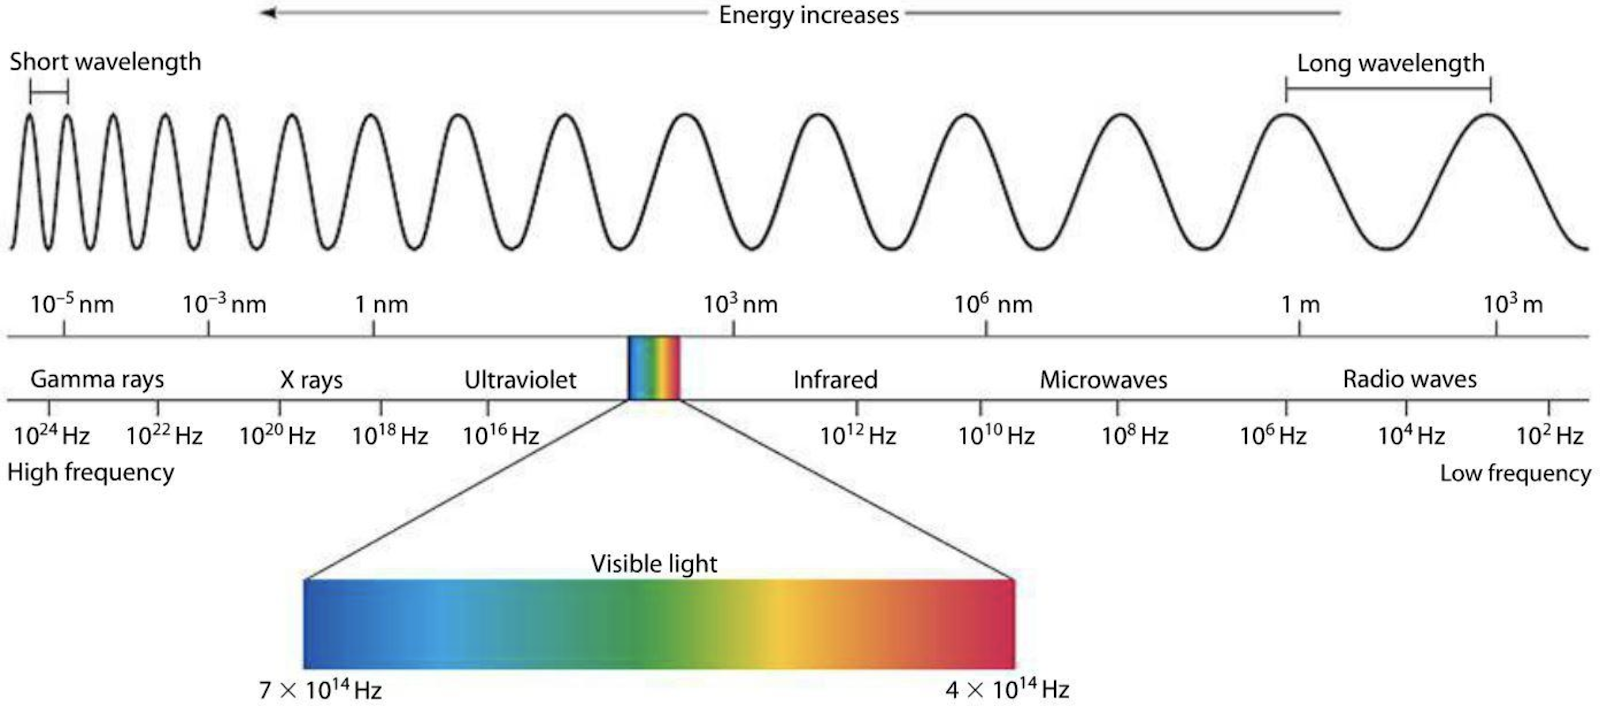
\includegraphics[width=0.8\linewidth]{img/electromagnetic_spectrum.png}
	\caption{An illustration of the electromagnetic spectrum~\cite{electromagneticSpectrum}} \label{fig:electromagneticSpectrum}
\end{figure}

In this thesis, we will focus on \emph{visible light}, which covers only a mere fraction of the electromagnetic spectrum. Its waves are roughly in the 380-780nm range.

To sum up, electromagnetic waves specify the way in which light travels. To, however, describe the interaction between light and matter, the term \emph{photon} is used. Photons are elementary particles of light moving in a manner specified by their wavelengths, making up electromagnetic radiation. They can be emitted or absorbed by atoms and molecules. During this process, they transfer energy either from the object that emitted them or to the object that absorbed them. This change in energy (denoted $E$) is proportional to the frequency of the absorbed/emitted photon and can be computed as follows~\citep{planckConstant}: 
\begin{equation} \label{energyEquation}
E = hf = \dfrac{hc}{\lambda}
\end{equation}
where $h$ is Planck's constant, $f$ is the frequency and $c$ is the speed of light. Therefore, generally speaking, the human eye identifies light when atoms and molecules in the retina absorb photons. 

To specify this process, we will first describe the retina. The retina consists of millions of light-sensitive cells, also called \emph{photoreceptors}, which pass a visual signal via an optic nerve to the brain, giving the notion of light and color. There are two types of photoreceptors in the human eye --- rods and cones.

\emph{Rods} make up most of the receptor cells (around 91 million according to~\citet{rods91cones4f5}, but other sources state that their number could be as high as 125 million~\cite{rods125cones6}). They are usually located around the boundary of the retina, and are responsible for low light (scotopic) vision. However, they possess very little notion of color, which is also the reason why the human eye has trouble recognizing colors during the night.

\emph{Cones} are located mainly in the center of the retina and their numbers are a lot lower (from around 4.5 million~\cite{rods91cones4f5} to 6 million~\cite{rods125cones6}). In contrast to rods, they are active at daylight levels (responsible for photopic vision) and have the notion of color. To be specific, different types of cones differ in their sensitivity to photon energies at concrete wavelengths. The final color is then composed by the brain from the stimulation signals sent by each cone.

The human eye has three types of cones:
\begin{itemize}
	\item \emph{L-cones}, which are the most responsive to longer wavelengths at around 560nm. When they are stimulated, they correspond to the red color.
	\item \emph{M-cones}, which are the most sensitive to medium wavelengths at around 530nm and correspond to green color
	\item \emph{S-cones}, which respond the most to small wavelengths that peak at around 420nm and correspond to blue color
\end{itemize}

Their relative response to stimulation can be seen in~\cref{fig:coneSensitivity}.
\begin{figure}[t]
	\centering
	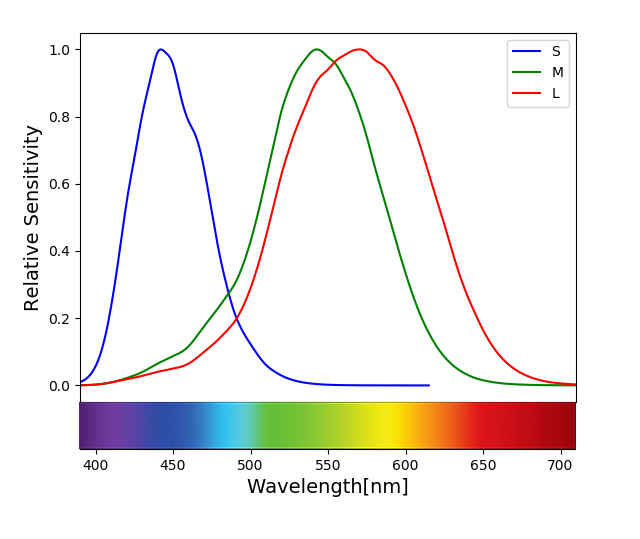
\includegraphics[width=0.5\linewidth]{img/cone_sensitivity.png}
	\caption{Relative sensitivity of S, M and L-cones plotted according to the data measured by~\citet{coneSensitivities}.} \label{fig:coneSensitivity}
\end{figure}

This type of color perception is called \emph{trichromatic}, as it uses three types of receptors to create the whole color space.

The idea behind using three base colors has been adapted in color science to create multiple tristimulus color representations. We will discuss these more thoroughly in the following section.

Up until now, we have been talking about the interaction of light with the human eye. Photons, however, also interact with objects. As established by the relationship defined in~\cref{energyEquation}, the energy transferred to an object upon light interaction is dependent on the photon wavelength. This means that objects might absorb some wavelengths and reflect others.

Object color is defined by the wavelengths it \emph{reflects}. For example, if it reflects all the wavelengths, the resulting color is white, while absorbing all the wavelengths would render the object black. Naturally, human perception of object color is not only dependent on its reflective properties, but also on the lighting of the scene. If the only light present in the scene is red, other wavelengths than red will never hit the object. Therefore, the object might reflect only a subset of wavelengths than it would under white light, which might change the resulting color.

\section{Color representation}

The question of how to discretely represent color has been posed ever since the introduction of the first graphical user interface. For use in computer science, representations are required to be compact, precise, and the operations on colors should be easily executed.

We have already briefly mentioned the tristimulus representation in the previous section. In this section, we will overview its basic properties and describe some of the most popular tristimulus systems. We will also talk about an alternative representation, based primarily on the physical properties of color --- spectral representation.

\subsection{Spectral representation}

When defining the color of an object, we must not only specify the wavelengths it reflects, but also the ratio between the incoming energy and the outgoing energy at these wavelengths. The dependence of reflectance on the wavelength is called a \emph{reflectance spectrum}, and is usually a smooth, continuous curve.

Although this definition might be sufficient for reflective surfaces, describing the color emitted by a light source requires the knowledge of the source's power rather than reflectance. For these purposes, \emph{spectral power distribution} (SPD) is used. Generally, SPD is a function describing the relationship between wavelength and any radiometric or photometric quantity (radiant energy, luminance, luminous flux, irradiance et cetera\ldots). In this thesis, we will use SPD to describe the emissive properties of light sources, and will therefore consider SPD to be a function of wavelength and power.

To compute the color of an object under a light source, one must simply combine the light source's SPD with the reflectance curve of the object, as shown in figure. This way the physical properties of color are preserved and the result is the same as it would be in nature, which, as we will show later, is not always the case with tristimulus representation.

\subsection{Tristimulus representation} \label{ssec:tristimulusRepres}

The obvious drawback of spectral representation is the difficulty of its discretization. Another, bigger problem, is caused by the fact that there is an infinite number of possible spectral curves, but only a discrete number of colors perceptible by human eye or even possible to generate by a computer (use word domain?). Representing colors with spectral distribution therefore requires their conversion to a discrete space before arbitrary visualization process.

Tristimulus representation skips the conversion steps and saves the already discretized color as a set of three values. Although the original idea was to simulate the trichromatic perception of human eye (i.e. save values that specify how much have the red, green and blue cones been stimulated), over time, multiple other tristimulus color spaces have been created. They differ mostly in the range of colors they are capable of representing and in their practical use. Following, we provide an overview of some of the most popular ones.

\subsubsection{RGB color space}
The RGB color space is an additive space employing three primaries --- red, green and blue. In other words, if you have three lights with red, green and blue chromacities respectively and you use them to illuminate a single point, you can create any color within the RGB color space solely by changing the lights' intensities. 

An RGB value can be therefore thought of as a point in a 3-dimensional euclidean space with each of the coordinate axes representing one of the primaries. Specifically, as the light's intensities must be bounded, we can narrow this space down to a cube starting at the base of the coordinate system. Usually, the range for each value is defined within 0 and 255, but a normalized (0,1) range is also used.

Various implementations of the RGB color space exist. They differ in the specifications of the RGB primaries, and therefore in their \emph{color gamut}, which is the subset of colors they are capable of representing. Some examples (named in ascending order with respect to their color gamut) include ISO RGB, sRGB, Adobe RGB, Adobe Wide Gamut RGB and ProPhoto RGB. An illustrative comparison of the sRGB and Adobe RGB gamut in the chromaticity diagram (described thoroughly in~\cref{sssect:xyYcolorSpace}) can be seen in~\cref{fig:chromaticityDiagram}.

RGB color spaces are commonly used in everyday world, e.g. in LCD and LED displays, digital cameras, scanners and even in computer graphics rendering. Their main downside has, however, been discovered when designing color matching functions~\cite{colorMatchingDerivation}.

A \emph{color matching function} is a function designed to simulate the response of a certain type of cone in the human eye. In 1931, CIE designed a set of three color matching functions that could be used for spectral to RGB conversion~\cite{colorMatchingDerivation}. Denoted $\overline{r}(\lambda)$, $\overline{g}(\lambda)$ and $\overline{b}(\lambda)$, they approximate the response of the L, M and S cones respectively. However, as seen in figure~\cref{fig:colorMatchingRGB}, the functions may also acquire negative values. This posed a problem at that time due to calculation errors. Therefore, to eliminate these negative portions of functions, CIE designed a new, imaginary color space --- the XYZ color space (tu ref?).

\begin{figure}[t]
	\centering
	\begin{subfigure}{0.46\textwidth}
		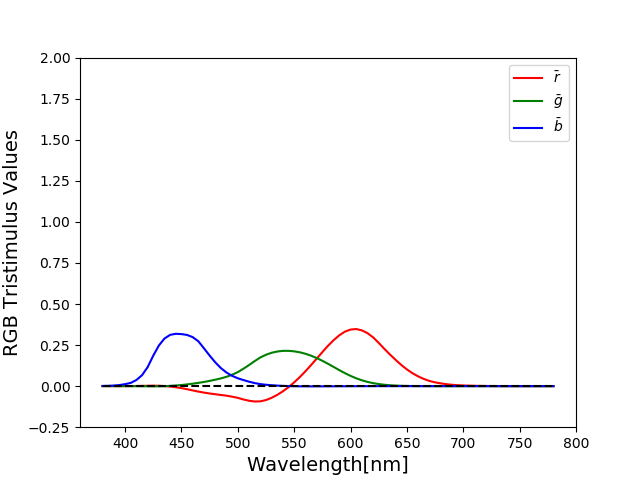
\includegraphics[width=\linewidth]{img/matching_functions_rgb.png}
		\caption{ $\overline{r}(\lambda)$, $\overline{g}(\lambda)$ and $\overline{b}(\lambda)$ functions plotted with data by~\citet{colorMatchingRGBData}}
		\label{fig:colorMatchingRGB}
	\end{subfigure}
	\quad
	\begin{subfigure}{0.46\textwidth}
		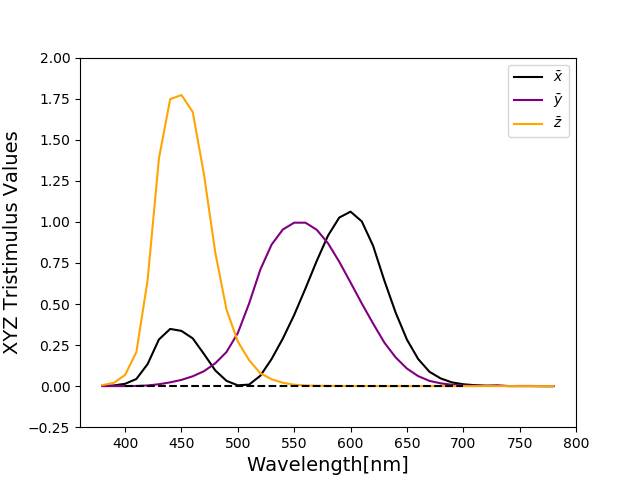
\includegraphics[width=\linewidth]{img/matching_functions_xyz.png}
		\caption{$\overline{x}(\lambda)$, $\overline{y}(\lambda)$ and $\overline{z}(\lambda)$ functions according to their spectral data from~\citet{colorMatchingXYZData}}
		\label{fig:colorMatchingXYZ}
	\end{subfigure}
	\caption{Color matching functions}
	\label{fig:colorMatchingFunctions}
\end{figure}

\subsubsection{XYZ color space}

The XYZ color space is a hypothetical color space capable of encompassing all colors perceptible by the human eye. Its color matching functions, $\overline{x}(\lambda)$, $\overline{y}(\lambda)$ and $\overline{z}(\lambda)$, were specifically designed for the purposes of SPD to tristimulus conversion, which is computed using the following equations:
\begin{equation} \label{spdToXYZ}
	\begin{aligned}
	X=\int P(\lambda)\overline{x}(\lambda)d\lambda,\\
	Y=\int P(\lambda)\overline{y}(\lambda)d\lambda,\\
	Z=\int P(\lambda)\overline{z}(\lambda)d\lambda,\\
	\end{aligned}
\end{equation}
where $X$, $Y$ and $Z$ are the resulting tristimulus values and $P(\lambda)$ is the spectral power distribution.

Although the X, Y and Z primaries were designed so that the Y primary closely matches luminance and X and Z primaries give color information, they are only imaginary, i.e. they do not correspond to any spectral distribution of wavelengths. This property renders the whole XYZ space imaginary, which means that it cannot be used for visualization purposes. Its main function is to therefore serve as a ``middle step'' when performing a conversion from SPD to an arbitrary tristimulus space, which eliminates the need for other color matching functions. The conversion from XYZ into a tristimulus space can then be performed by a simple space-specific $3x3$ matrix transformation.

\subsubsection{xyY color space} \label{sssect:xyYcolorSpace}

In addition the impossible visualization process, another downside of the XYZ color space is that its values are practically unbounded and do not have any real meaning (such as the RGB triplets have). Therefore, a more intuitive color space has been created, which considers the relative proportions of the X, Y and Z values rather than their unbounded versions --- the xyY color space~\cite{xyYOverview}. It is based on the assumption that color can be regarded as a quantity with two properties: \emph{luminance} and \emph{chromaticity}.

First, the following conversion from the $X$, $Y$ and $Z$ values to their bounded versions, also called \emph{chromaticity coordinates}, is performed~\cite{xyYEquations}:
\begin{equation} \label{XYZtoxyY}
\begin{aligned}
&x=\dfrac{X}{X+Y+Z}\\
&y=\dfrac{Y}{X+Y+Z}\\
&z=\dfrac{Z}{X+Y+Z}\\
\end{aligned}
\end{equation}
Due to normalization ($x+y+z=1$), $z=1-x-y$, which means that we can drop the term $z$ from the representation as it does not give any additional information about the current color. It also implies that we lost some information during the conversion --- we cannot reconstruct the original XYZ triplet using only two values $x$ and $y$ and therefore cannot obtain the initial color. At least one of the original values is needed for this purpose ---~\citet{CIE} decided to use the $Y$ component, as it already specifies the luminance.

Plotting the values of the $x$ and $y$ components creates a \emph{chromaticity diagram}, shown in~\cref{fig:chromaticityDiagram}. Each point of the curved boundary line (which is also called the \emph{spectral locus}) corresponds to a XYZ value that is the result of a monochromatic radiation (i.e. a single-wavelength stimulus). All other chromaticities visible to the standard observer lie within a region bounded by the spectral locus.

\begin{figure}[t!]
	\centering
	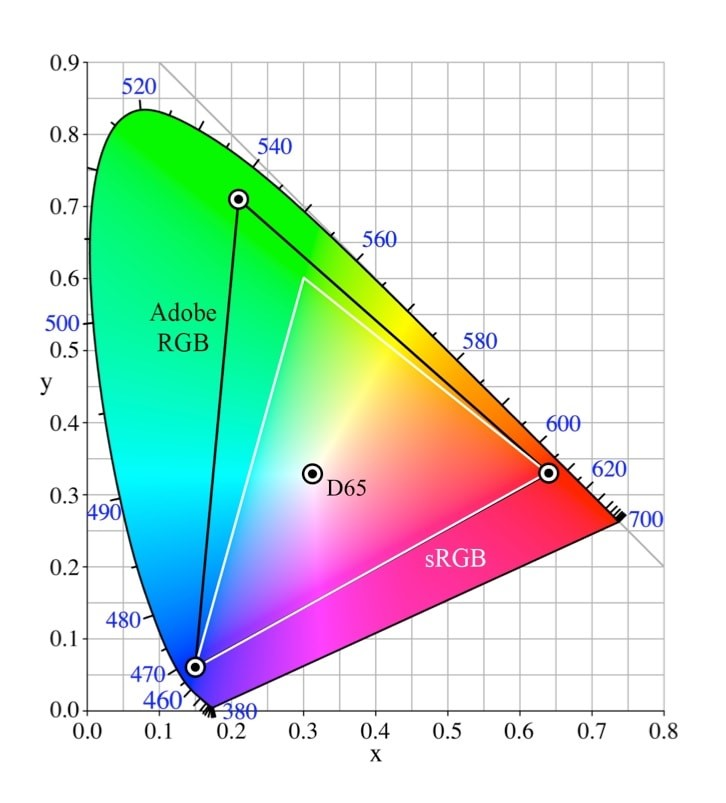
\includegraphics[width=0.6\linewidth,height=0.3\textheight]{img/chromaticity_diagram.jpeg}
	\caption{An illustrative comparison of the sRGB and Adobe RGB gamut in the chromaticity diagram based on images created by~\citet{chromaticityDiagramResource}}
	\label{fig:chromaticityDiagram}
\end{figure}

\subsubsection{L*a*b*}

Although the xyY color space is already much more intuitive in terms of human color perception, the differences between individual triplets of the system are not perceptually uniform. The Hunter's Lab color space ref addressed this issue and was designed so that the distance between its two triplets characterized roughly how different they are in chromaticity and luminance. It is based on the Opponent color theory~\cite{opponentColorTheory}, which suggests that the cones in the human eye are linked together in opposing pairs and that the visual system records the \emph{difference} between the stimulation of the pairs rather than the cones' individual responses.

As the Hunter's Lab color space does not achieve perfect uniform spacing of values, CIE \emph{L*a*b*} color space (CIELAB) has been proposed in an attempt to improve some of its shortcomings and is now more widely used. However, neither of the systems are completely accurate in terms of perceptual uniformity~\cite{hunterLabCIELabComparison}.

The three opponent channels used to specify color in the CIE L*a*b* color space are defined as follows~\cite{labColorScale}:
\begin{itemize}
	\item \emph{L*} --- indicates lightness, i.e. the difference between \emph{light} and \emph{dark}. Its values range from $0$ (yielding black color) to $100$ (indicating diffuse white color)~\cite{labColorScale}.
	\item \emph{a*} --- defines the difference between \emph{green} and \emph{red}. Positives values of this component indicate the object's color to be more green, while negative values indicate red.
	\item \emph{b*} --- defines the difference between \emph{yellow} and \emph{blue}. Positive values indicate the object to be more yellow, while negative values indicate blue.
\end{itemize}
Neither the range of the a* nor the b* component has any specific numerical limits~\cite{labColorScale}.

The L*a*b* color space is a \emph{reference system} --- an abstract, non-intuitive space encompassing all the human perceptible colors. Due to its perceptual uniformity, it is used for color balance corrections by modifying the a* and b* components, and for lightness adjustments by modifying the L* component. 

Another advantage and common use of the L*a*b* color space is for computing \emph{color differences}. In 1976, CIE introduced the concept of \emph{Delta E}, which is the measure of change in visual perception of two colors~\cite{deltaEOverview}. Denoted $\Delta E_{ab}^*$, it is computed as an Euclidean distance between the two sample points, i.e.:
\begin{equation} \label{deltaE}
\Delta E_{76}=\sqrt{(L_{2}^* - L_{1}^*)^2 + (a_{2}^* - a_{1}^*)^2 + (b_{2}^* - b_{1}^*)^2},
\end{equation}
where $(L_{1}^*,a_{1}^*,b_{1}^*)$  and $(L_{2}^*,a_{2}^*,b_{2}^*)$ are the L*a*b* coordinates of the sample points.

However, the sensitivity of the human eye to color differences is not uniform. It is, for example, more sensitive to small color differences in dark blue colors than it is in e.g. light pastel colors. The $\Delta E_{ab}^*$ error does not take this ununiformity into account and therefore shows exaggerates differences in light colors while compressing perceptual distances between darker colors. To improve upon these shortcomings, other measuring techniques for computing Delta E have been proposed over the years, such as Delta94 and Delta2000.

\emph{Delta94} is computed by modifying the original L*a*b* values of both colors to compensate for perceptual distortions in the color space and computing Euclidean distance from the new modified values. Although the results match the human color difference perception more closely, the Delta94 error metric still lacks some accuracy in the blue-violet region~\cite{deltaEOverview}.
	
\emph{Delta2000} attempts to remove these inaccuracies. Along with the corrections added to Delta94, Delta2000 adds overall five correctional factors to the original $\Delta E_{ab}^*$ --- compensation factors for lightness, hue and chroma, compensation for neutral colors and, lastly, a hue rotation term for the problematic blue-violet regions. 

From the listed Delta E equations, the Delta2000 error measurements are the most accurate in terms of human color difference perception~\cite{deltaEOverview} and, therefore, will also be used in the practical parts of this thesis. However, as the specifics of the Delta2000 equations are out of scope of this thesis, we refer the interested reader to the original article by~\citet{delta2000}.

\subsubsection{Other color spaces}

In addition to the already named tristimulus color spaces, there exist many more used for various purposes. Following, we briefly overview some of them:
\begin{itemize}
\item \emph{L*u*v*} --- Similarly to the CIELAB system, L*u*v* (or CIELUV) aims for perceptual uniformity. As a matter of fact, the $L*$ value is defined in the same manner as in the CIELAB system, while $u$ and $v$ values are evaluated by certain projections of the $x$ and $y$ coordinates of the chromaticity diagram. When comparing their Euclidean error measure, the most important distinction between the two spaces is that while  CIELAB generally improves CIELUV in terms of color difference~\cite{CIELABcomparisonCIELUV}, CIELUV does not have as many inaccuracies in the dark regions~\cite{CIELABDarkSide}. Therefore, it is often recommended to use the CIELUV color space for characterization of color displays and CIELAB color space for the characterization of colored surfaces and dyes.

\item \emph{HSL} and \emph{HSI} color spaces define color by its \emph{hue}, \emph{saturation} and \emph{lightness} (or \emph{intensity}). They are an alternative representation of the RGB color space and must therefore be defined purely with reference to an RGB space~\cite{HSLreview}. As their components correlate better with human perception of color than those of the RGB system, they are often used in image processing applications, e.g. for processes such as feature detection (edge detection~\cite{edgeDetectionHSL}, object recognition) or image segmentation (which can be performed solely with/by? the hue component)~\cite{HSLreview}.

\item \emph{CMYK} model is a subtractive color model commonly used in color printing. It is based on RGB's complementary colors --- \emph{cyan}, \emph{magenta} and \emph{yellow} respectively. This means that assigning zero values to all components renders white light, and increasing the value of a component specifies how much of the respective color is \emph{subtracted} from the white light. Although the theory states that maximizing CMY values should render perfect black, in reality, the printing inks are not 100\% CMY and their combinations cannot produce rich black. For this purpose, a fourth component, \emph{black} ($K$), is often added, giving rise to the CMYK model.

\end{itemize}

Other color spaces include Munsell color system, RAL, Natural Color System, Pantone Matching System, CIELCH\textsubscript{ab}, CIELCH\textsubscript{uv}, etc$\ldots$

\subsection{Color representation in rendering}

Accurate color representation is the core of rendering softwares. Although most of today's renderers support multiple color spaces, we can still divide them into two main categories according to the space used during evaluation of light transfer equations --- \emph{tristimulus} and \emph{spectral} renderers.

Tristimulus renderers are usually based on the RGB color space, although they often offer conversions to other tristimulus spaces. Due to the ease of use and simplicity of representation, RGB renderers are more common in commercial rendering software. They provide realistically looking images, often indistinguishable from a photograph, and are more robust, easy to implement and memory efficient.

\begin{figure}[t]
	\centering
	{\sffamily
		\begin{tabular}{cc}
			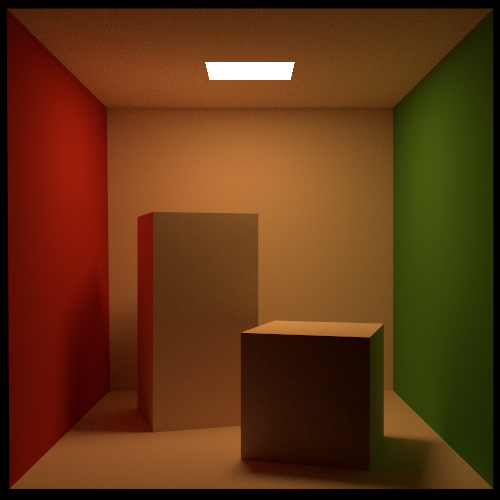
\includegraphics[width=0.45\linewidth]{img/mitsuba_rgb_mode.jpg}
			&
			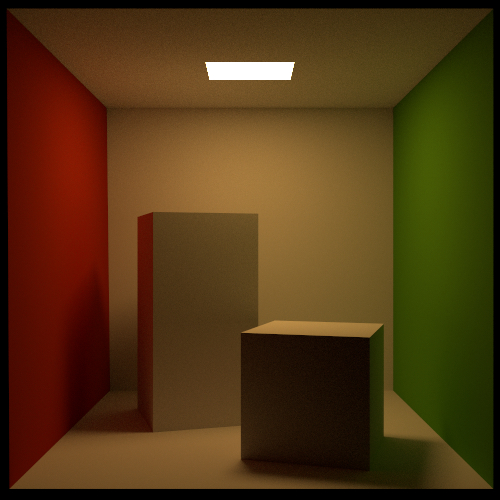
\includegraphics[width=0.45\linewidth]{img/mitsuba_spectral_mode.jpg}\\
		\end{tabular}
	}
	\caption{Comparison of an RGB-based rendering and spectral-based rendering as presented in the documentation of Mitsuba2~\cite{Mitsuba2}. Left: Spectral reflectance data of all materials is first converted to RGB and the scene is then rendered in the RGB mode, producing an unnaturally saturated image. Right: Scene is rendered directly in the spectral mode, resulting in more realistic colors. }
	\label{fig:mitsubaRGBSpectralComparison}
\end{figure}

However, light in real world does not travel as a tristimulus value, but rather as a distribution of wavelengths. As RGB renderers do not possess full-spectral information of materials and light in the scene, they cannot properly simulate the physical properties of the color during e.g. reflections or refractions when ray tracing.

Spectral rendering, on the other hand, uses full-spectral information of all materials and light in the scene during the whole rendering process. Obviously, before visualization occurs, spectral information must be converted into tristimulus (usually RGB) values, but this does not pose a problem as, at the moment of conversion, all the physically-based simulations have already taken place. Therefore, the rendered scene appears more realistic. We demonstrate this difference in~\cref{fig:mitsubaRGBSpectralComparison}, on a scene already rendered by Mitsuba2~\cite{Mitsuba2}.

In addition to rendering reflections and refractions more convincingly, another reason for using spectral rendering is its capability of simulating physically based phenomena that arises due to the interaction of color with light. Following, we overview some of the most common ones:
\begin{itemize}
\item \emph{Metamerism} \label{item:metamerism}

As already mentioned in~\cref{ssec:tristimulusRepres}, the human tristimulus perception has a significantly lower domain than the (practically infinite) spectral domain. Therefore, two different spectra can trigger the same cone response in the human eye and appear to have the same color (and, subsequently, to have the same RGB values), giving rise to a phenomenon called \emph{metamerism}. The two spectra evaluating to the same tristimulus values are called \emph{metamers}.

In real world, metamerism is often perceived when the lighting conditions under which we observe metamers change. An example of this can be seen in~\cref{fig:metamerism}, where the color of the presented spheres under the D65 illuminant is similar, while it clearly differs under the fluorescent F11 illuminant.

Obviously, this behavior is irreproducible by an RGB renderer, as it cannot replicate the behavior of spectral reflectance under an illuminant.

\begin{figure}[t]
	\centering
	{\sffamily
		\begin{tabular}{cccc}
			Sphere reflectance curve & D65 Illuminant & F11 Illuminant 
			\vspace{1em} \\
			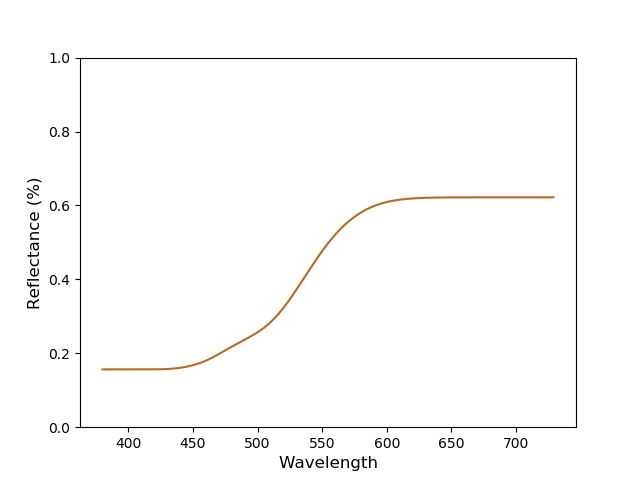
\includegraphics[width=.30\linewidth]{img/metamerism_first_curve.png}
			&
			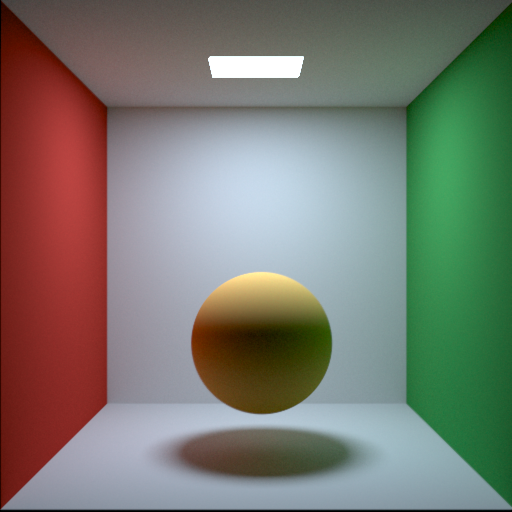
\includegraphics[width=.30\linewidth]{img/metamerism_first_d65.png}
			& 
			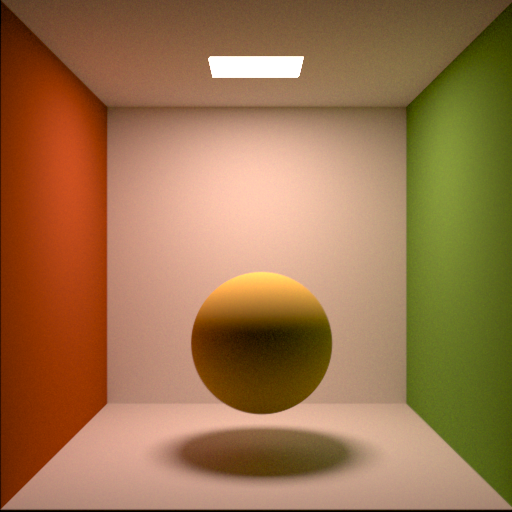
\includegraphics[width=.30\linewidth]{img/metamerism_first_fl11.png}
			\vspace{1em} \\
			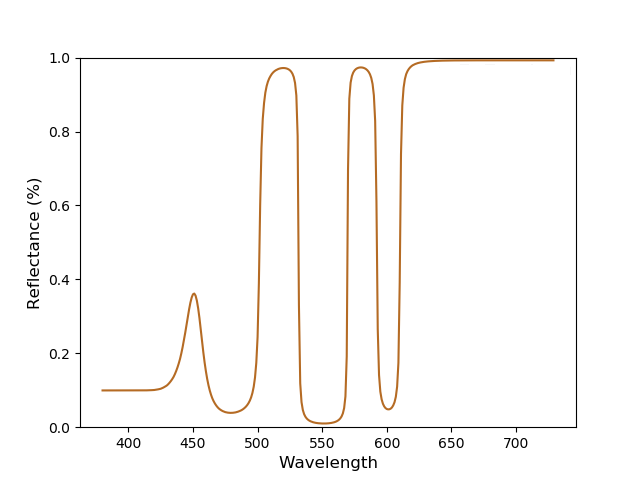
\includegraphics[width=.30\linewidth]{img/metamerism_second_curve.png}
			&
			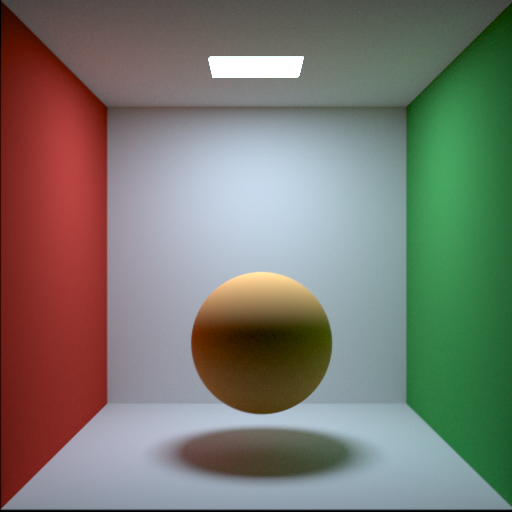
\includegraphics[width=.30\linewidth]{img/metamerism_second_d65.png}
			&
			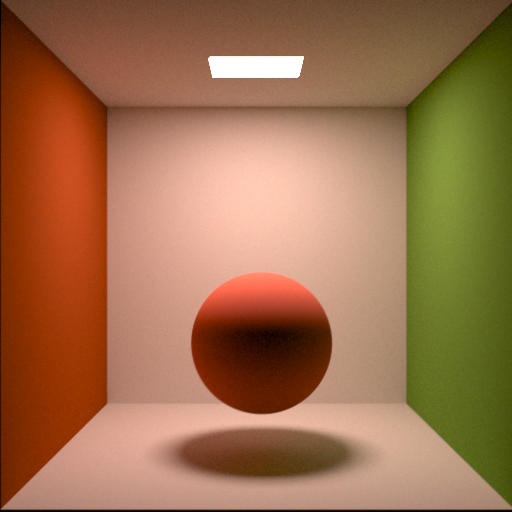
\includegraphics[width=.30\linewidth]{img/metamerism_second_fl11.png}
		\end{tabular}
	}
	\caption{The effects of metamerism. Left: Two different spectral reflectance curves, both evaluating to roughly $RGB=(220,175,105)$ under D65. Middle and right: Renderings of a sphere with assigned reflectance curves under D65 and F11 illuminants}
	\label{fig:metamerism}
\end{figure}


\item \emph{Fluorescence}

By definition, fluorescence occurs when light from one excitation wavelength $\lambda_0$ is absorbed by an object and is almost immediately re-emitted at a different, usually longer, wavelength $\lambda_1$~\cite{fluorescenceDefinition}. Specifically interesting is the fact that the absorbed light can come from outside of the visible spectrum and be re-emitted inside it, which results in unrealistically bright material appearance, perceivable in real world when for example fish, corals, jellyfish or even minerals are illuminated by a UV light.

RGB renderers attempt to fake this kind of behavior it through custom shaders~\cite{fluorescencePolarization}. As it produces satisfactory results and is immensely easier to implement than physical simulation, physically based fluorescence has received small amount of work. Its support can be found in spectral renderers, added for example to ART by~\citet{fluorescenceART}.

\item \emph{Iridescence}

\emph{Iridescence}, or goniochromism, is a phenomenon occurring when certain surfaces change their color according to the current viewing angle. It arises when the object's physical structure causes interferences between light waves (e.g. inside extremely thin dielectric layers), yielding rich color variations~\cite{iridescenceArticle1}. It can be perceived in nature in certain plants, specific minerals, butterfly wings, peacock's feathers, snakes, but also in man-made products such as oil leaks, soap bubbles or car paints.

Similarly to fluorescence, iridescent behavior can be ``faked'' in an RGB renderer~\cite{iridescenceRGB}. However, research based on physical properties of iridescence has also been conducted. For further information about the current development, we refer the interested reader to the articles by~\citet{iridescenceArticle1},~\citet{iridescenceArticle2}, or~\citet{iridescenceArticle3}.

\item \emph{Dispersion}

When light travels from one medium to another (e.g. when light hits glass or water), its direction of travel is changed. This phenomenon is called \emph{refraction} and is closely described by Snell's law, which specifies how the angle of refraction can be computed from the angle of incidence and the \emph{refraction indices} of the two media~\cite{snellsLaw}. However, the refraction index depends not only on the \emph{type} of media, but also on the current \emph{wavelength}~\cite{dispersionRendering1} --- which implies that the resulting direction of photons of different wavelengths might vary.

Probably the most popular example of this phenomena is white light hitting a dispersive prism. Upon interaction, light is split into a spectrum, creating a ``rainbow'' effect.

There have been multiple attempts to simulate physically-based dispersion. We refer the interested reader to articles by~\citet{dispersionRendering1} or~\citet{dispersionRendering2}.

\item \emph{Polarization}

Electromagnetic waves traveling through space are \emph{transverse waves} --- their oscillation is perpendicular to their path of propagation. By default, the directions of oscillations are arbitrary for each photon --- this type of light is called an \emph{unpolarized light}. Restrictions to the directions of oscillations (also called \emph{polarization}) render \emph{polarized light}. Such phenomenon usually occurs upon light's interaction with certain materials.

The polarization process contributes to the overall color only in special cases (e.g. when using polarization filters)~\cite{fluorescencePolarization}. Therefore, it receives little attention in implementation of rendering softwares. However, for physical consistencies (and due to the possibility of special scenes) both ART~\cite{ART} and Mitsuba~\cite{Mitsuba2} follow the direction of oscillation during the rendering process.
\end{itemize}

Other researched phenomena (some of it closely linked to the already mentioned ones) include \emph{phosphorescence}, \emph{bioluminescence}, \emph{dichroism}, \emph{opalescence}, \emph{aventurescence} and many more.

